% LTeX: language=fr
%%%%%%%%%%%%%%%%%%%%%%%%%%%%%%%%%%%%%%%%%%%%%%%%%%%%%%%%%%%%%%%%%%%%%%%%%%

%%%%%                           Conclusion Géné                     %%%%%%
%%%%%%%%%%%%%%%%%%%%%%%%%%%%%%%%%%%%%%%%%%%%%%%%%%%%%%%%%%%%%%%%%%%%%%%%%%


\phantomsection 
\addcontentsline{toc}{chapter}{Conclusion générale}
\addtocontents{toc}{\protect\addvspace{10pt}}

\vspace*{-1cm}
\section*{\fontsize{24pt}{24pt}\selectfont\textnormal{~~~~~~~Conclusion générale}}
\vspace{2cm}

\lhead[\fancyplain{}{Conclusion et perspectives}]
      {\fancyplain{}{}}
\chead[\fancyplain{}{}]
      {\fancyplain{}{}}
\rhead[\fancyplain{}{}] 
      {\fancyplain{}{Conclusion et perspectives}}
\lfoot[\fancyplain{}{}]
      {\fancyplain{}{}}
\cfoot[\fancyplain{}{\thepage}]
      {\fancyplain{}{\thepage}}
\rfoot[\fancyplain{}{}]
     {\fancyplain{}{\scriptsize}}

%%%%%%%%%%%%%%%%%%%%%%%%%%%%%%%%%%%%%%%%%%%%%%%%%%%%%%%%%%%%%%%%%%%%%%%%%%
%%%%%                      Start part here                          %%%%%%
%%%%%%%%%%%%%%%%%%%%%%%%%%%%%%%%%%%%%%%%%%%%%%%%%%%%%%%%%%%%%%%%%%%%%%%%%%

%/!\/!\/!\/!\/!\/!\/!\/!\/!\/!\/!\/!\/!\/!\/!\/!\/!\/!\/!\/!\/!\/!\/!\/!\
\subsection*{Synthèse des travaux}
\label{sec:conclu_Synthese des travaux}
%/!\/!\/!\/!\/!\/!\/!\/!\/!\/!\/!\/!\/!\/!\/!\/!\/!\/!\/!\/!\/!\/!\/!\/!\

Les travaux dont le présent mémoire a fait l'objet s'inscrivent dans le cadre de l'amélioration de l'autonomie des batteries des appareils d'aide à l'audition. Ils ont permis l'élaboration d'une nouvelle architecture optimisée de récupérateur d'énergie dédiée à la valorisation optimale de l'énergie de déformation mécanique du conduit auditif, résultant des mouvements de la mâchoire.\\

Nous avons tout d'abord établi un état de l'art autour des méthodes d'optimisation des performances et de l'intégrabilité des applications nomades sur du corps humain. Nous avons notamment ciblé leur besoin énergétique et montré la pertinence de la récupération de l'énergie dissipée par les activités du corps humain dans ce cadre. Les verrous technologiques introduits par le contexte applicatif sur les systèmes de récupération ont été mis en avant, ainsi que les solutions apportées par la littérature. Plus particulièrement, nous avons montré que l'autonomie énergétique des appareils d'aide à l'audition pouvait être améliorée en exploitant la déformation mécanique du conduit auditif à l'aide d'une démarche méthodique au regard des solutions d'optimisation existantes.

Le second chapitre introduit alors le récupérateur hydro-piézoélectrique amplifié à conversion \emph{frequency-up} visant à maximiser l'énergie récupérable depuis la déformation mécanique basse fréquence du conduit auditif. L'énergie est tout d'abord captée par un bouchon d'oreille moulé sur mesure et pressurisé sous fluide incompressible. Devenant ainsi une pompe avec les mouvements de la mâchoire qui le déforment, le bouchon transmet l'énergie hydraulique simultanément à deux pistons hydrauliques au travers d'un découpleur hydraulique, un amplificateur hydraulique et deux valves hydrauliques. Dans une première phase de fonctionnement, un des pistons pousse la masse dynamique d'un oscillateur bistable depuis une de ses positions d'équilibre stable jusqu'à sa position d'équilibre instable. Dans une seconde phase, la masse bascule alors vers la position d'équilibre stable symétrique et oscille jusqu'à l'arrêt. L'oscillateur intègre un générateur piézoélectrique, constitué d'un flextenseur et d'un empilement de céramiques PZT, capable de convertir une partie de l'énergie vibratoire de la masse dynamique en électricité. Le système est conçu pour cycler le mouvement de la masse, alternativement d'une position stable à l'autre, pour chaque fermeture de la mâchoire. À cet effet, nous avons introduit une nouvelle solution technologique de valves hydrauliques, basée sur le flambement en flexion de tubes flexibles, permettant de diriger le fluide sortant du bouchon d'oreille alternativement vers un des pistons, puis l'autre. Le cyclage du système est alors autonome, car le pilotage de l'ouverture des valves est assuré directement par la position de la masse dynamique. Le comportement multiphysique couplé des différents éléments est ensuite mis en équation et un modèle numérique est établi pour en étudier son comportement et avoir une première estimation des performances du système qui promet alors, en théorie, un rendement de conversion global de $67$\%, avec un rendement de $79$\% pour le convertisseur électromécanique haute fréquence seul. De plus, la simulation système permet d'extraire le cahier des charges hydraulique des valves en imposant un rapport minimal $(r_{Cf})_{min}$ de 10 entre les pertes de charges hydrauliques de la branche fermée et celles de la branche qui actionne.

Le chapitre trois décrit la caractérisation expérimentale du convertisseur électromécanique composé de l'oscillateur bistable implémentant le générateur piézoélectrique. Un modèle EF a été alors établi pour son dimensionnement et sa conception tente de pallier les éventuels défauts pouvant être introduits durant sa fabrication. Un banc de caractérisation spécifique est mis en \oe{}uvre et les résultats expérimentaux sont corrélés au modèle théorique. Une nette différence entre les performances attendues et mesurées est observée, puisque le rendement du convertisseur électromécanique seul est estimé expérimentalement à $12.9$\%. Ce résultat pourrait provenir des légères ondulations locales des lames de l'oscillateur bistable, produites par sa fabrication et sa manipulation, mais aussi des imperfections de montage, induisant une réduction du facteur de qualité et du coefficient de couplage du convertisseur électromécanique. Malgré la baisse de rendement, son comportement dynamique s'avère conforme à celui du modèle théorique.

Le chapitre quatre présente une approche expérimentale visant à dimensionner et concevoir les valves hydrauliques assurant le cyclage de la masse de l'oscillateur bistable. La valve est fabriquée en kapton pour sa grande résistance mécanique et sa souplesse offerte par de très faibles épaisseurs. Un banc de test statique a été mis en \oe{}uvre pour caractériser la raideur en rotation d'échantillons de tubes en kapton. Une méthode de plastification locale y est utilisée, dans le but de réduire cette raideur, tout en conservant les fonctionnalités de la valve. Un banc de test hydraulique motorisé a été enfin mis en \oe{}uvre dans le but de caractériser les pertes de charges au travers de la section flambée des tubes kapton, en fonction de l'angle de flexion imposé. Le tube remplissant le critère statique du cahier des charges de la valve est alors caractérisé sur le banc hydraulique et il se révèle capable d'assurer le rapport $(r_{Cf})_{min}=10$ pour le bon cyclage de la masse. Par ailleurs, nous avons caractérisé le comportement cinématique de la valve, intégrée sur l'oscillateur bistable, en fonction des mouvements de la masse. Nous avons notamment souligné l'influence positive des gaines rigides autour du tube kapton et nous avons établi les nouveaux systèmes d'équations liant la position de la masse à l'angle de flexion de la valve. 

La répétabilité du processus de plastification rendant difficile la prédiction du comportement statique des valves, le chapitre cinq propose une approche théorique pour leur modélisation et leur dimensionnement. La caractérisation des pertes de charges, en fonction de l'angle de flexion post-flambement pour des tubes flexibles, n'existe pas, à notre connaissance, dans la littérature. La géométrie complexe de la section flambée est alors approximée à une réduction, suivie d'une expansion conique, ce qui nous donne une relation entre le diamètre hydraulique à la section flambée du tube et le coefficient de pertes de charges qui est lié. Additionné au cahier des charges hydraulique de la valve, cela nous a aidé à calculer le diamètre hydraulique nécessaire à la section flambée, en fonction du diamètre initial du tube, pour assurer sa fermeture du point de vue de l'écoulement. Il reste alors à déterminer l'angle de flexion nécessaire pour atteindre le diamètre hydraulique de fermeture. Cela nous a mené à établir un modèle EF du tube kapton afin d'étudier les comportements cinématique et statique durant sa flexion. Une prospection préliminaire a révélé que pour maximiser l'étranglement hydraulique il faut maximiser le diamètre du tube, en minimisant son épaisseur. En revanche, pour minimiser sa raideur en rotation, minimiser son diamètre et surtout son épaisseur. Le couplage du modèle analytique de pertes de charges avec les données du modèle EF permettent de vérifier si un tube spécifique répond au cahier des charges hydraulique et statique de fonctionnement d'une valve. Enfin, les résultats du modèle théorique sont confrontés aux données expérimentales du chapitre précédent sur les deux aspects. Les ordres de grandeurs et les tendances des raideurs post-flambement des tubes sont similaires sur l'aspect statique. Le modèle théorique prédit des raideurs plus importantes avant le flambement, à cause notamment des conditions limites du modèle qui n'incluent pas le contact mécanique extérieur de la masse. De plus, les tendances sur l'aspect hydraulique sont similaires, mais les ordres de grandeurs théoriques sont nettement plus faibles devant les données expérimentales. Les différences sont notamment dues à l'hypothèse de simplification géométrique qui semble trop éloignée de la réalité. Le modèle théorique du comportement des valves n'est donc pas encore suffisamment prédictif pour être utilisé pour un dimensionnement, c'est pourquoi le modèle global sera complété préférablement avec les données expérimentales.

Dans le dernier chapitre, nous rassemblons les données de caractérisations expérimentales de l'oscillateur bistable, du générateur piézoélectrique et des valves hydrauliques pour l'établissement d'un modèle plus réaliste du comportement du récupérateur présenté dans cette thèse. Nous mettons d'abord en avant la réduction de la bistabilité de l'oscillateur sous l'influence de la raideur croissante des valves. Suite à cela, nous donnons une méthode de redimensionnement du système mécanique solidaire composé des deux organes valve + oscillateur, afin de préserver l'énergie pouvant y être emmagasinée durant la poussée du piston. De plus, nous présentons les essais de caractérisations dynamiques du comportement oscillatoire de la masse sous l'influence des frottements contre la valve. Un modèle de frottement sec est introduit pour caractériser la dissipation énergétique au contact entre les deux composants. Un processus essais-erreurs permet ensuite, grâce au modèle système numérique, d'estimer la valeur du coefficient de frottement sec à $0.42$ suite aux essais expérimentaux. Le rendement du convertisseur est finalement évalué à $2.6$\%. Par ailleurs, nous avons établi l'influence des paramètres du système sur ses performances. La complexité du couplage entre les paramètres est alors mise en évidence par les compromis devant être faits pour maximiser le rendement, en s'assurant que la dynamique du système soit préservée. Enfin, des pistes d'améliorations sont proposées pour améliorer le modèle prédictif, ainsi que pour réduire les dissipations énergétiques au contact entre la masse et la valve. \\
\newline 
\textbf{Synthèse de ce que le modèle global permet d'anticiper :}
\begin{itemize}[label=$\circ$]
      \item Le couplage multiphysique entre tous les composants du système.
      \item La variabilité du niveau énergétique d'entrée.
      \item L'influence des valves hydrauliques à base de tubes flexibles sur le comportement statique et dynamique du convertisseur électromécanique.
      \item Les pertes de charges nécessaires dans une branche hydraulique pour favoriser l'écoulement vers l'autre branche.
      \item Le rendement de conversion énergétique de l'oscillateur bistable implémentant le générateur piézoélectrique, sous l'influence mécanique d'une valve hydraulique.
      \item L'influence des différents paramètres de réglage sur le rendement de conversion global, mais aussi sur le fonctionnement du système.
\end{itemize}
\textbf{Synthèse de ce que le modèle global ne permet pas d'anticiper :}
\begin{itemize}[label=$\circ$]
      \item Le rendement de conversion énergétique des composants qui n'ont pas été étudiés durant la thèse, à savoir, le découpleur et l'amplificateur hydraulique.
      \item La réponse, en débit et en pression, du bouchon d'oreille face à l'impédance mécanique non linéaire de l'oscillateur bistable.
      \item La variabilité des amplitudes d'ouverture et de fermeture de la mâchoire pour un individu donné.
\end{itemize}

%/!\/!\/!\/!\/!\/!\/!\/!\/!\/!\/!\/!\/!\/!\/!\/!\/!\/!\/!\/!\/!\/!\/!\/!\
\subsection*{Perspectives}
\label{sec:conclu_Perspectives}	
%/!\/!\/!\/!\/!\/!\/!\/!\/!\/!\/!\/!\/!\/!\/!\/!\/!\/!\/!\/!\/!\/!\/!\/!

Ce doctorat a permis d'évaluer la faisabilité d'une nouvelle architecture de récupérateur d'énergie pour une source mécanique basse fréquence. Les résultats présentés introduisent par ailleurs des perspectives pouvant donner suite à ces travaux.\\

Le dimensionnement du système passe actuellement par de nombreux outils numériques tels que ANSYS mechanical, ANSYS Workbench, Matlab, Simulink ou LabVIEW. L'influence des paramètres multiphysiques sur le comportement du système a été établie dans la thèse, mais il serait intéressant de mettre en \oe{}uvre une méthode d'optimisation capable de calculer les paramètres de réglage optimaux du dispositif, en fonction de l'énergie disponible et du critère de confort imposés. Cela permettrait, d'une part, de faciliter et accélérer la démarche de développement et de compréhension du système, et d'autre part, de réduire les incertitudes sur les résultats de corrélations modèle-essais.\\

Le modèle prédictif du comportement hydraulique des tubes flexibles flambés gagnerait en précision dans une étude dédiée au sujet. La fabrication de valves sans adaptateurs de diamètre réduirait par exemple les incertitudes de mesure sur le coefficient de pertes de charges dans une approche expérimentale. L'approche théorique pourrait également gagner en précision à l'aide d'un modèle mécanique des fluides numérique couplé au modèle éléments finis statique établi dans le chapitre cinq.\\

Le comportement du bouchon d'oreille est par ailleurs assimilable à celui d'une pompe. Cela ouvre un grand champ d'applications diverses pour le système développé dans nos travaux. Sa complexité rend favorable son utilisation pour des dimensions importantes et pour des densités de puissance d'entrée plus importantes, car alors le système peut s'affranchir des restrictions confort, de fragilité et d'encombrement.

Les surpressions dans les circuits hydrauliques (canalisations urbaines, industrielles, etc.) sont des causes récurrentes de l'endommagement des composants hydrauliques, mais aussi de la rupture des conduites \cite{Koutnik2006,Flemming2009}. Le système hydrau-électromécanique développé ici pourrait servir d'absorbeur avec un découpleur hydraulique réglé sur le seuil de pression maximal admissible dans la conduite. Une mise en parallèle de multiples dispositifs réglés à des seuils de pression différents pourrait optimiser l'absorption. De plus, l'énergie générée pourrait servir à l'alimentation de capteurs autonomes autour du dispositif.

Par ailleurs, la force du système réside dans la transformation d'une "force" à sens unique, en une "force" dans deux sens opposés. Cela donne accès à des sources d'énergies intéressantes pour l'autonomie de dispositifs nomades. Par exemple, un bouton poussoir connecté pourrait être alimenté par la seule force générée par la pression sur celui-ci. Aussi, une balance autonome pourrait être alimentée par la force générée lorsque l'utilisateur monte dessus.



% Théoriquement $K_{T40}$ diminue quand $\theta_{VH}$ augmente. Nous allons nous mettre dans le cas défavorable où $K_{T40} = K_{T40}(\ang{25})$ sur la plage d'angle $\Delta \theta _{25,50}$ pour l'intégration au modèle système. Sur la figure \ref{fig:Ep et F_elas en fonction de x_m} on va retrouver l'évolution de l'énergie potentielle et de la force élastique contenus dans le système, en fonction la position de M. Les trois différentes courbes correspondent respectivement à :
%  On constate à travers la figure \ref{fig:Ep et F_elas en fonction de x_m} que l'impact de la VH est significatif sur le comportement mécanique de l'OB. En revanche, le système \{OBVH\}$_{eq}$ redimensionné a un comportement statique et énergétique quasi-similaire à l'OBs. En effet, on s'aperçoit que pour une même barrière de potentiel, l'\{OBVH\}$_{eq}$ admet une position d'équilibre stable légèrement supérieure à celle que l'OBs. La conséquence sera visible sur le volume de fluide nécessaire pour la course des pistons qui sera d'autant plus importante que cet écart augmentera.\\
% 	Nous allons donc calculer les nouveaux paramètres du système \{OBVH\}$_{eq}$ dont le fonctionnement nécessite le même niveau d'entrée énergétique que celui de l'OBs.
% %%%%%%%%%%%%%%%%%%%%%%%%%
% \begin{figure}[!htbp]
% \begin{center}
% 	\begin{subfigure}[b]{0.48\textwidth}
%     	\captionsetup{justification=centering}
% 		\includegraphics[trim={8cm 0cm 0cm 0cm},clip, 					                 width=\textwidth]{../Chap5/Figure/Ep__{OB seul}_{OBVH}_{OBVH_eq} .pdf}
% 		\caption{Impact de $K_{T40}(\ang{25})$ sur l'énergie potentielle de M}
% 		\label{fig:(Ep)_vs_(x_m)_avec_(K_VH)}
% 	\end{subfigure}
% \hfillx
% 	\begin{subfigure}[b]{0.48\textwidth}
%     	\captionsetup{justification=centering}
% 		\includegraphics[trim={8cm 0cm 0cm 0cm},clip, 					                 width=\textwidth]{../Chap5/Figure/Felas__{OB seul}_{OBVH}_{OBVH_eq} .pdf}
% 		\caption{Impact de $K_{T40}(\ang{25})$ sur la force élastique de M}
% 		\label{fig:(F_elas)_vs_(x_m)_avec_(K_VH)}  
% 	\end{subfigure}
% 	\caption{Impact de $K_{T40}(\ang{25})$ sur le comportement mécanique de l'OB}
% 	\label{fig:Ep et F_elas en fonction de x_m}
% \end{center}	
% \end{figure}
% %%%%%%%%%%%%%%%%
% Grâce au système d'équation \ref{eq:x0_eq}, on sait que pour que la barrière de potentiel du nouveau système \{OBVH\}$_{eq}$ et  soit équivalente à celle de l'OBs flambé à $x_{0,l}=0.49$mm, il faudra lui appliquer une hauteur de flambement initiale de $x_{0eq}=0.6$mm avant que la VH ne s'ajoute. Ce paramètre est critique à déterminer car sa valeur doit rester plus faible que $x_{0m}$ pour assurer un couplage électromécanique optimal et une intégrité structurelle lors des oscillations de M. Cela accorde la validité au tube T40 sur le critère énergétique de VH.\\
% Ayant vérifié que le comportement hydraulique, ainsi que l'impact mécanique théorique du tube T40 soient en adéquation avec le cahier des charges attendu pour une VH, nous allons l'intégrer au modèle système global pour simuler une nouvelle fois le comportement du récupérateur durant plusieurs cycles de mastication.
%     %///////////////////////////////////////////// 		
% 	\subsection{Simulation du modèle système comprenant les valves}
% 	\label{subsec:6.3.3_Simulation du modèle système comprenant les valves}
%     %/////////////////////////////////////////////	    
% 	Nous avons réalisé des simulations avec le nouveau modèle implémentant le comportement mécanique et hydraulique du tube T40 utilisé avec un décalage d'angle de \ang{30}. En entrée du système nous avons utilisé le même relevé de données de l'évolution du débit entrant et sortant du bouchon d'oreille qu'on retrouve sur la figure \ref{fig:debit_ear}. Les données ont été concaténées à l'identique afin de simuler plusieurs cycles de mastication identiques.\\
% 	Nous avons recalé la hauteur de flambement $x_{0,eq}$ de l'OB${eq}$ de façon à ce que la barrière de potentiel à franchir par M avec l'influence de la VH reste identique à celle de l'OBs flambé initialement à $\tilde{x_0}$. De cette façon l'amplification hydraulique reste aussi identique au modèle précédent. Les tableaux \ref{tab:OB_seul} et \ref{tab:recalage_OBVH} mettent en parallèle les valeurs numériques des paramètres de l'OBs utilisé lors du pré-dimensionnement dans le chapitre \ref{ch:3}, avec celles du modèle \{OBVH\}$_{eq}$ recalé, implémentant l'impact théorique du tube T40 sur la plage d'angle $\Delta\theta_{25,50}$.\\
% %%%%%%%%%%%%%%%%%%%%%%%%%%%%%%%%%%%%%%%%%%%%%%%%%%%%%      
% \def \hfillx {\hspace*{ -\textwidth} \hfill}
% \begin{table}[!htbp]
% 	\begin{minipage}[t]{0.45\textwidth}
% 	\centering	
% 	\rowcolors[]{2}{black!8}{}{
% 		\begin{tabular}[t]{m{2.5cm} | c | c }
% 		\rowcolor{blue!10}
% Paramètre & Symbole & Valeur \\
% \hline
% \hline
% Flambement OBs             & $x_{0,l}$             &  0.49mm \\ 
% Fermeture VH               & ${(r_{cf})}_{min}$   & 10 \\ 
% Rendement global           & $\eta_{gs}$          & 67\% \\
% Position initiale 
% piston   		           & $xp_{0s}$            & 0.78mm \\
% Amplification hydraulique  & $h_{0s}$             & 6 \\
% \hline
% 		\end{tabular}}
%         \caption{Paramètres de l'OBs}
%         \label{tab:OB_seul}
% 	\end{minipage}
% %\hfillx
% 	\begin{minipage}[t]{0.45\textwidth}
% 	\centering
% 	\rowcolors[]{2}{black!8}{}{
% 		\begin{tabular}[t]{m{3.5cm} |c| c}
% 		\rowcolor{blue!10}
% Paramètre & Symbole & Valeur \\
% \hline
% \hline
% Flambement OB$_{eq}$       & $\tilde{x_{0}}$       &  0.6mm \\ 
% Flambement \{OBVH\}$_{eq}$ & $x_{0,eq}$ 		   &  0.5mm \\ 
% Rigidité VH                & $K_{T40}(\ang{25})$   & 0.38Nmm/rad \\ 
% Coude VH       		       & $a_{eq}$ 			   & 1.2mm \\
% Fermeture VH   			   & $r_{cf,eq}$			   & 17 \\ 
% Rendement global 		   & $\eta_{g,eq}$	       & 68\% \\
% Position initiale 
% piston   		           & $xp_{0,eq}$           & 0.78mm\% \\
% Amplification hydraulique  & $h_{eq}$              & 6 \\
% \hline
% 		\end{tabular}}
%         \caption{Paramètres du système \{OBVH\}$_{eq}$}
%         \label{tab:recalage_OBVH}
% 	\end{minipage}
% \end{table}
% %%%%%%%%%%%%%%%%%%%%%%%%%%%%%%%%%%%%%%%%%
% Sur la figure \ref{fig:simulink_verif_tube__position_debit_Cf_pression_2CYCLES} on peut voir en concordance de temps, l'évolution des positions, débits, coefficients de PdC et pression en jeu.  On constate donc que l'étranglement généré au travers de la section flambée du tube T40 assure une gestion du débit adéquate permettant à M de réaliser un cycle complet. Rappelons que le mouvement oscillatoire sur $Cf_{VH}$ durant les oscillations de M est la conséquence du fait que le modèle prend comme considération que la VH est solidaire avec M durant cette phase. 
% %%%%%%%%%%%%%%%%%%%%%%%%%%%%%%%%%%%%	
% \begin{figure}[!htb]
% \begin{center}
%     \captionsetup{justification=centering}
% 	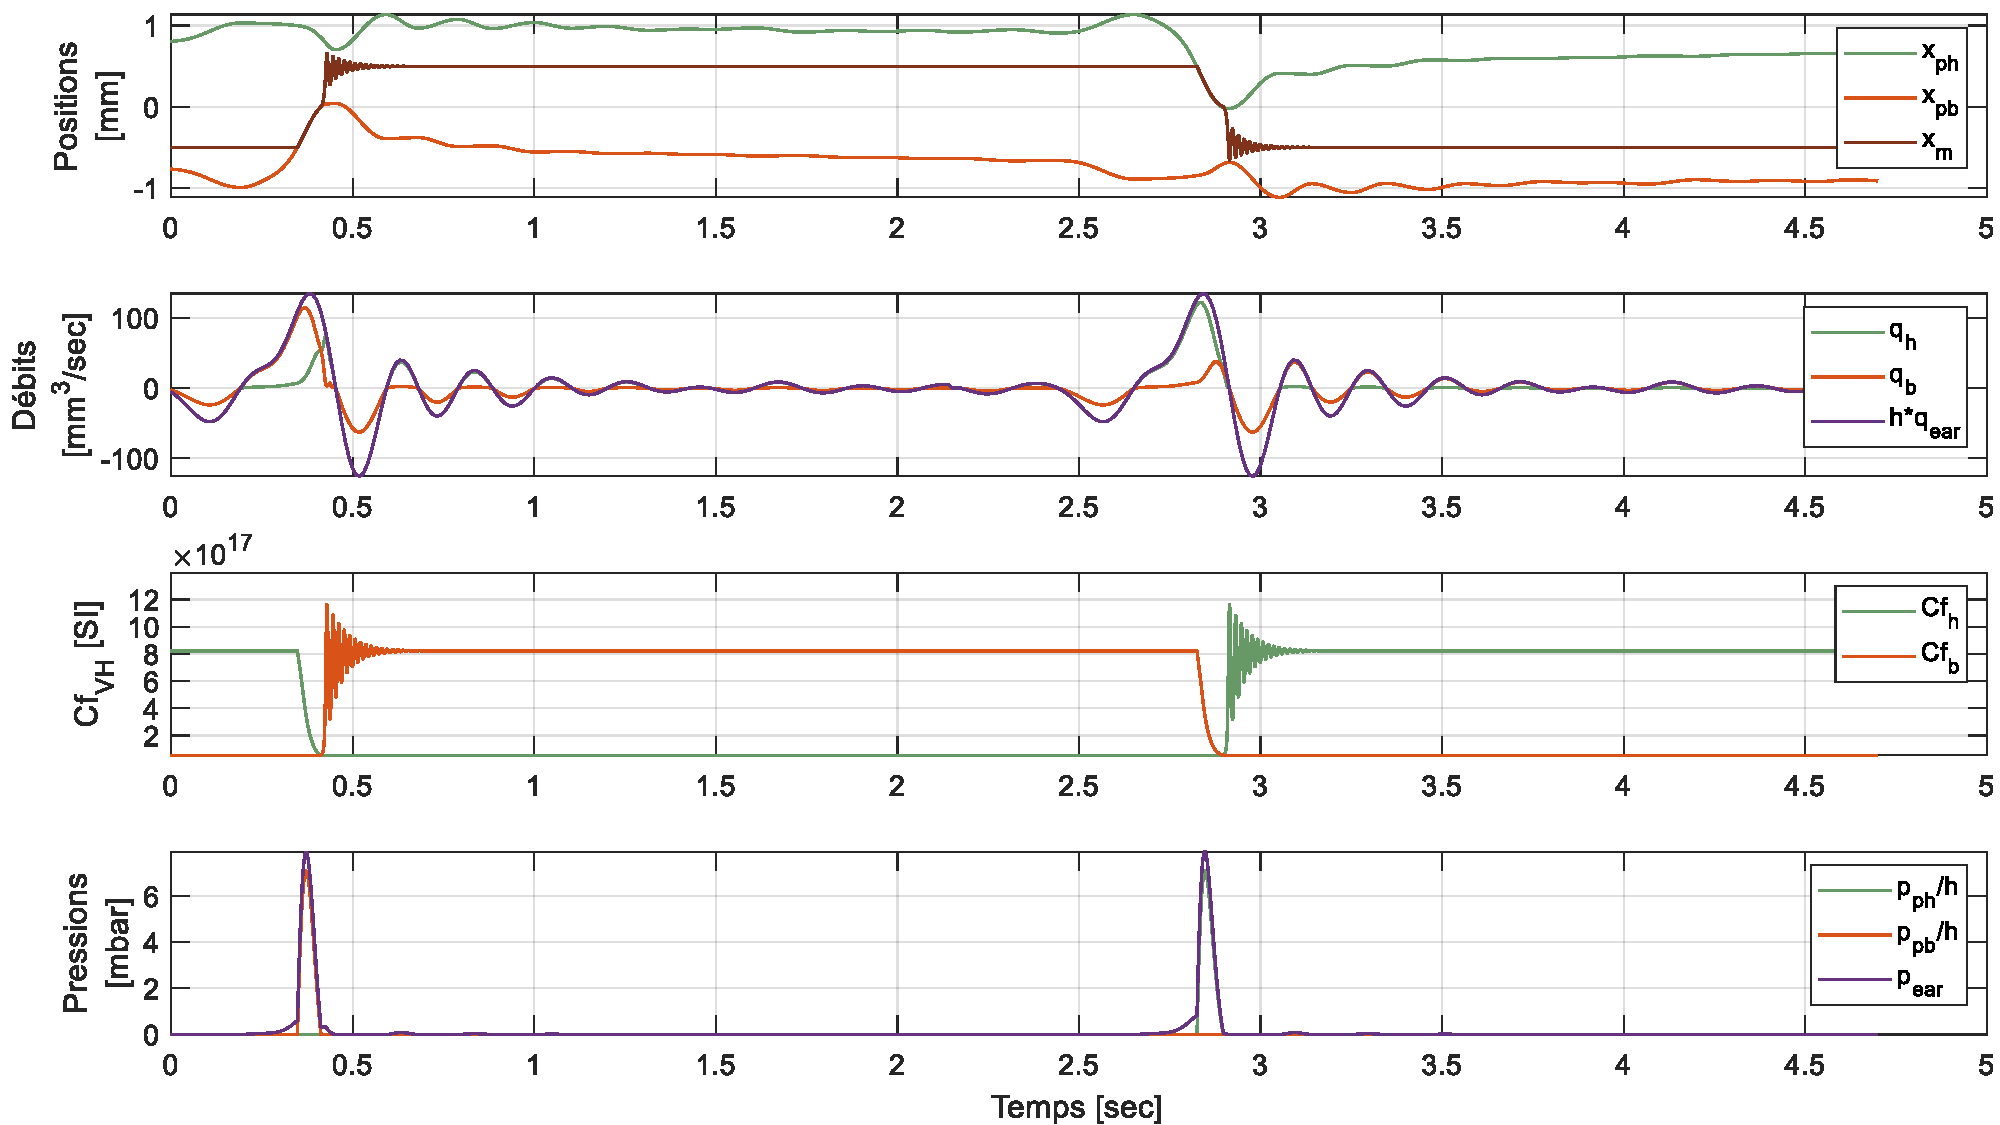
\includegraphics[trim={0cm 0cm 0cm 0cm},clip, 					                 width=\textwidth]{../Chap5/Figure/simulink_verif_tube__position_debit_Cf_pression_2CYCLES.pdf}
% 	\caption{Résultats de simulation pour les positions, débits, coefficients de PdC et pressions en concordance de temps - 2 cycles avec $K_{T40}(\ang{25})$}
% 	\label{fig:simulink_verif_tube__position_debit_Cf_pression_2CYCLES}
% \end{center}	
% \end{figure}    
% %%%%%%%%%%%%%%%%%%%%%%%%%%%%%%%%%%%% 
% Une différence notable avec le modèle précédent est remarquable sur le rapport de fermeture qui devant être d'un minimum de 10, a été choisi égal à 17 sur l'\{OBVH\}$_{eq}$. Cela s'explique par le profil de l'évolution de $Cf_{VH}$ avec la variation de $x_m$. On peut tracer sur la figure \ref{fig:comparaison_Cfcdc_Cfvh} $Cf_{VH}(x_m)$ pour les deux cas du cahier des charges et celui du tube T40 implémenté dans \{OBVH\}$_{eq}$. À l'équation \ref{eq:Cf=Cf0+csim*x} nous avons montré la relation linéaire entre $x_m$ et $Cf$ dans le cas du cdc. Aussi, la combinaison des équations \ref{eq:Cf_definition}, \ref{eq:theta=f(x_m)} et \ref{eq:Cf_Gibson_45deg} montre bien que la loi d'évolution $Cf(x_m)$ nous aide à tracer les points correspondants aux propriétés hydrauliques du tube T40. Nous avons défini $r_{cf}$ comme le rapport entre le coefficient de PdC quand M est en équilibre et celui quand la masse est en 0. Celui-ci ne tient donc pas compte de la vitesse d'étranglement de la section flambée lors de la flexion, mais seulement de la position fermée et ouverte du la valve. La figure \ref{fig:comparaison_Cfcdc_Cfvh} montre alors bien que lorsque M se rapproche de 0, les pertes de charges du modèle du T40 en position fermée sont plus faibles que celui du modèle linéaire.
% %%%%%%%%%%%%%%%%%%%%%%%%%%%%%%%%%%%%	
% \begin{figure}[!htb]
% \begin{center}
%     \captionsetup{justification=centering}
% 	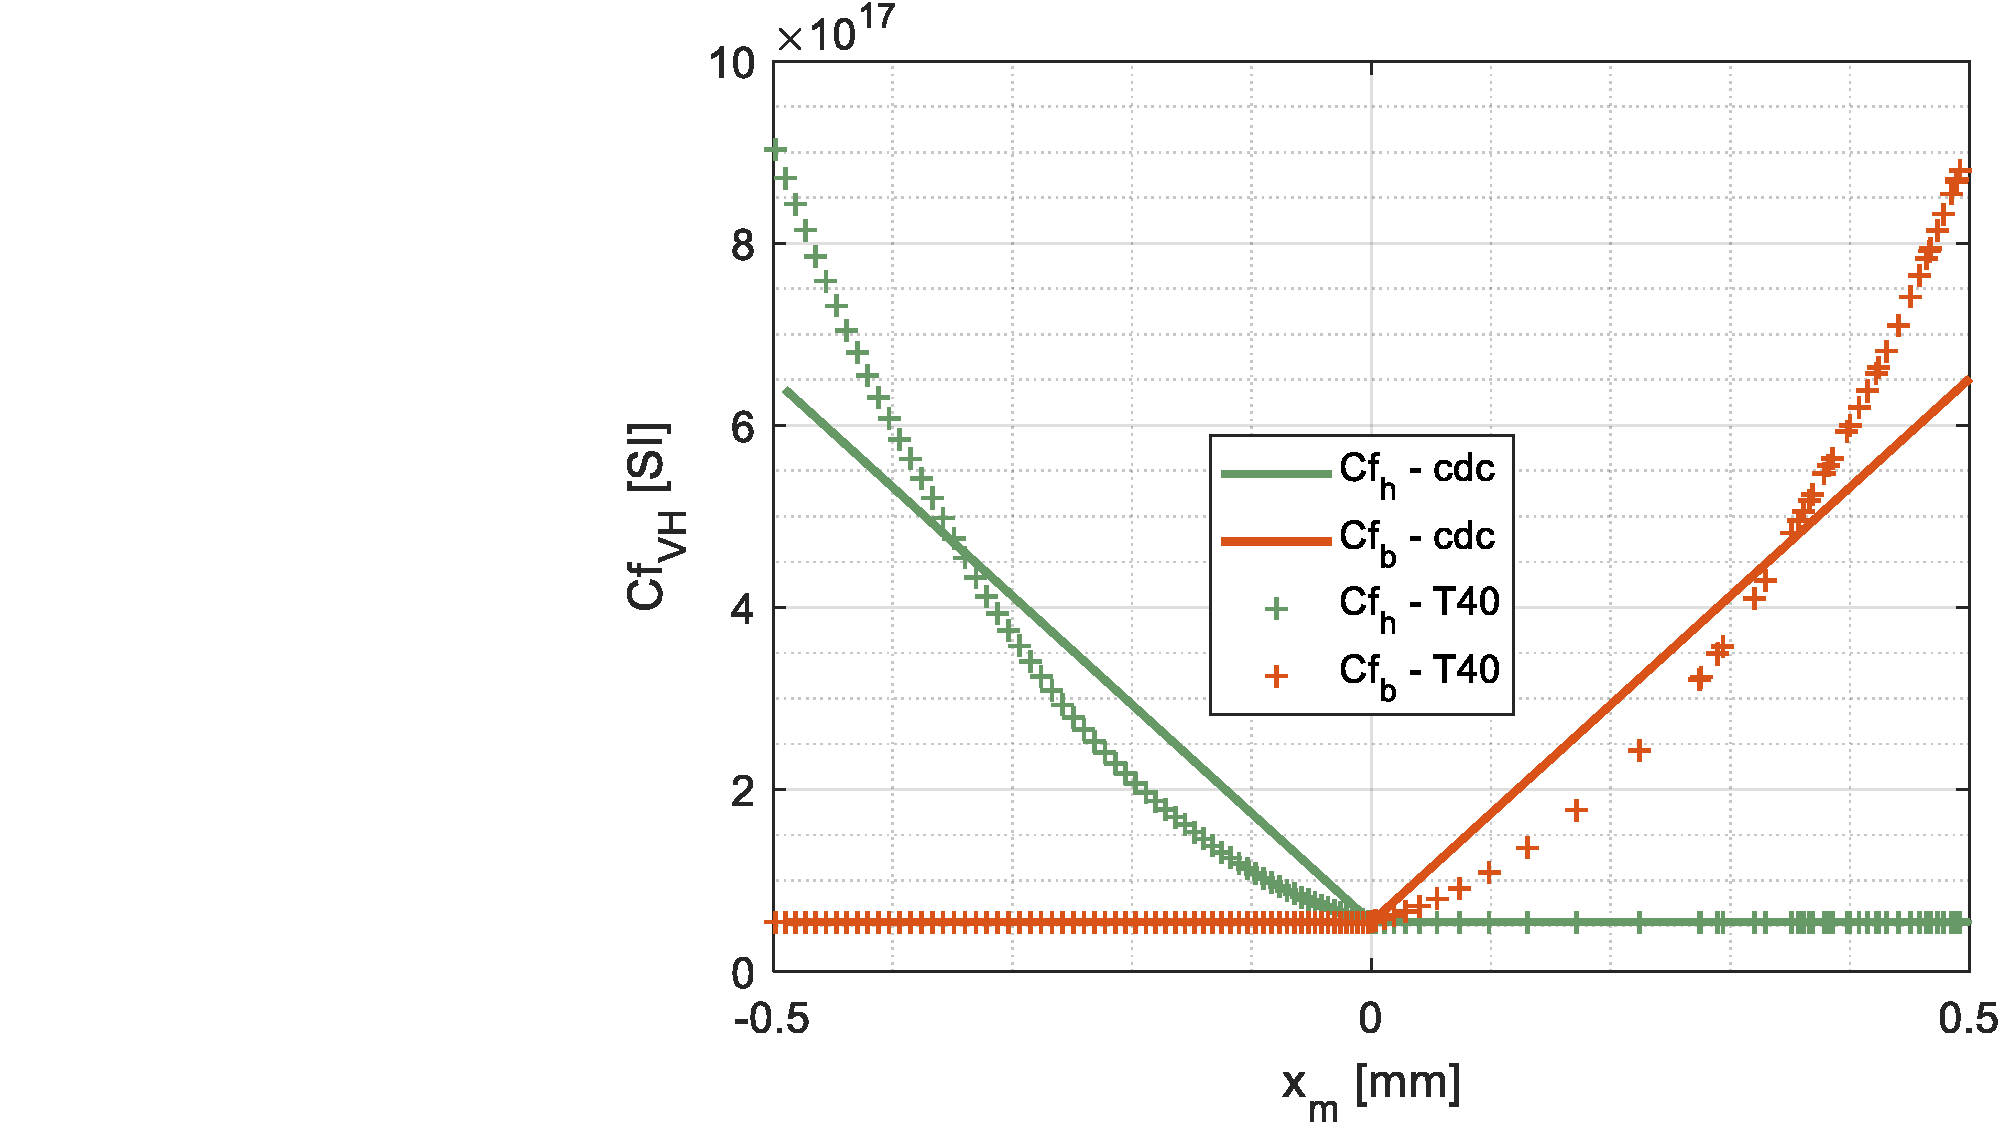
\includegraphics[trim={10cm 0cm 0cm 0cm},clip, 					                 width=0.6\textwidth]{../Chap5/Figure/comparaison_Cfcdc_Cfvh.pdf}
% 	\caption{Comparaison $Cf_{VH}(x_m)$ pour le cdc et le tube T40}
% 	\label{fig:comparaison_Cfcdc_Cfvh}
% \end{center}	
% \end{figure}    
% %%%%%%%%%%%%%%%%%%%%%%%%%%%%%%%%%%%% 
% D'autre part, si on regarde  la figure \ref{fig:simulink_verif_tube__position_debit_Cf_pression_1CYCLE}, elle montre l'évolution des mêmes paramètres que la figure précédente mais seulement durant le premier cycle de mastication. On y voit alors que le débit sortant du bouchon d'oreille est le plus important lorsque M est proche de 0. Combiné au constat précédent, le piston fermé recevra plus de débit durant l'actionnement dans le modèle \{OBVH\}$_{eq}$ que dans le modèle ayant servi au pré-dimensionnement. Comme nous savons que le volume $\Delta V_{ear}$ déplacé du bouchon d'oreille est limité, il nous faut nous assurer que le piston actif reçoit assez de fluide pour accomplir sa course jusqu'à 0. C'est pourquoi nous sommes contraints d'augmenter le rapport de fermeture à un minimum de 17 sur ce modèle, en sous duquel il est impossible d'assurer le mouvement alternatif du M.\\
% %%%%%%%%%%%%%%%%%%%%%%%%%%%%%%%%%%%%	
% \begin{figure}[!htb]
% \begin{center}
%     \captionsetup{justification=centering}
% 	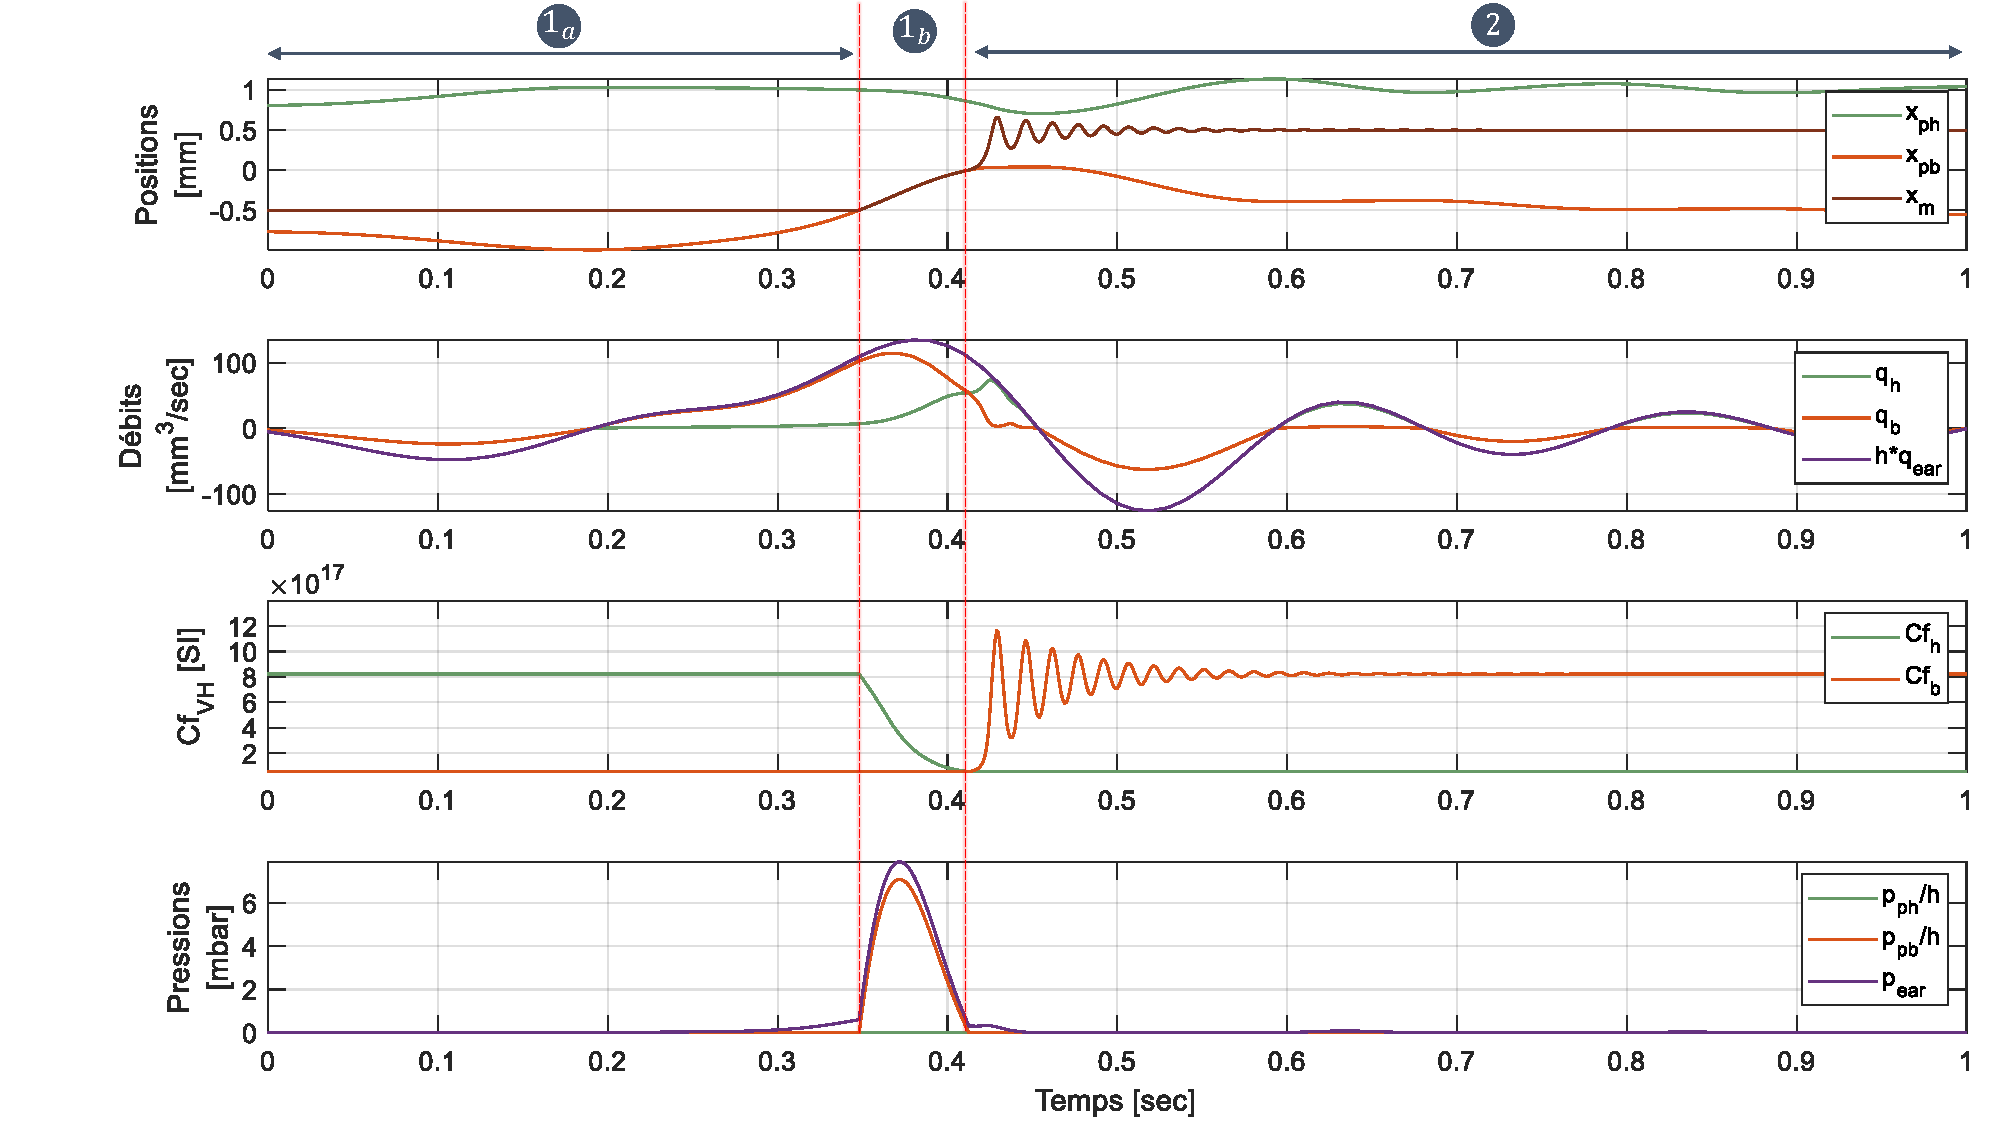
\includegraphics[trim={1.8cm 0cm 0cm 0cm},clip, 					                 width=\textwidth]{../Chap5/Figure/simulink_verif_tube__position_debit_Cf_pression_1CYCLE.pdf}
% 	\caption{Résultats de simulation pour les positions, débits, coefficients de PdC et pressions en concordance de temps - 1 cycle avec $K_{T40}(\ang{25})$}
% 	\label{fig:simulink_verif_tube__position_debit_Cf_pression_1CYCLE}
% \end{center}	
% \end{figure}    
% %%%%%%%%%%%%%%%%%%%%%%%%%%%%%%%%%%%% 	
% 	En addition, sur la figure \ref{fig:simulink_verif_tube__position_Up_puissance_energie_1CYCLE} on pourra retrouver en concordance de temps les aspects électriques et énergétiques du système. Cela comprend la tension du GPA, les puissances d'entrée et de sortie, ainsi que le bilan énergétique. En faisant le parallèle avec la figure \ref{fig:simu_pos_Up_puissances_energie_1CYCLE}, on s'aperçoit que le comportement du système est très semblable au premier modèle dimensionné sans le pliage du tube. Cela parait cohérent et confirme que nous avons réussi à corréler de façon adéquate les paramètres entre les deux modèles \{OBVH\}$_{eq}$ et OBs, comme on peut le voir dans les tableaux des valeurs des paramètres introduit plus haut. La résistance de charge de 15.5k$\Omega$ est restée identique à celui utilisé dans le modèle précédent.\\
% %%%%%%%%%%%%%%%%%%%%%%%%%%%%%%%%%%%%	
% \begin{figure}[!htb]
% \begin{center}
%     \captionsetup{justification=centering} 
% 	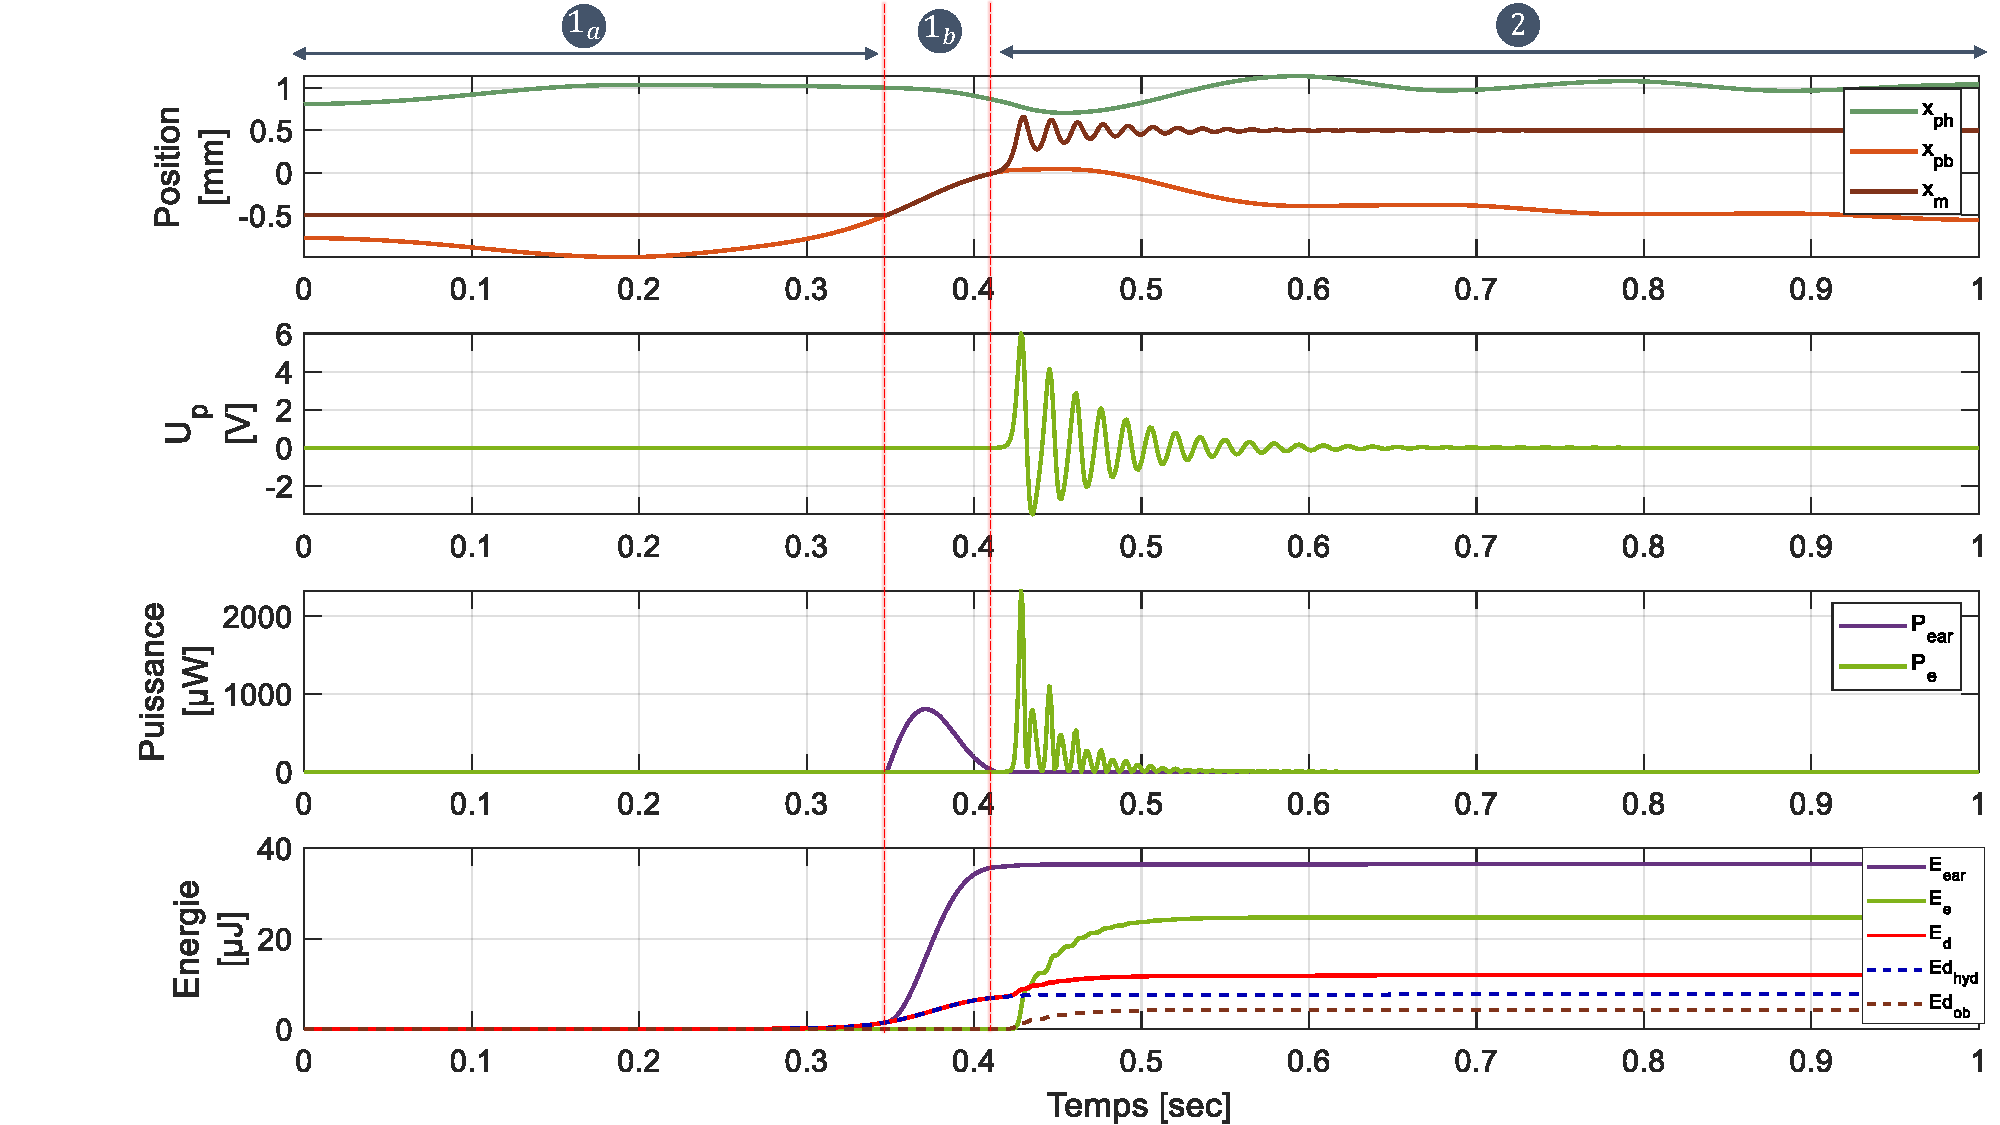
\includegraphics[trim={2cm 0cm 0cm 0cm},clip, 					                 width=\textwidth]{../Chap5/Figure/simulink_verif_tube__position_Up_puissance_energie_1CYCLE.pdf}
% 	\caption{Résultats de simulation pour les positions, tension GPA, puissances et énergies - 1 cycle avec $K_{T40}(\ang{25})$}
% 	\label{fig:simulink_verif_tube__position_Up_puissance_energie_1CYCLE}
% \end{center}	
% \end{figure}    
% %%%%%%%%%%%%%%%%%%%%%%%%%%%%%%%%%%%% 
% 	 On retrouve alors les 3 mêmes phases de fonctionnement $1_a$, $1_b$ et $1_c$ durant un cycle de mastication. Le GPA étant inchangé, on retrouve aussi les mêmes niveaux de tension et de puissance que lors du pré-dimensionnement. Les pertes hydrauliques durant l'actionnement de M sont elles aussi toujours prépondérantes devant les pertes mécaniques dans l'OB. Celles-ci sont directement liées à la plage d'angle que nous choisissons pour le fonctionnement de la VH. En effet, plus $\theta(x_m=0)$ est important, plus les pertes de charges dans le piston actif seront importants. Il pourrait être intéressant alors de les diminuer au maximum. Cependant, plus  $\theta(x_m=0)$ est faible, et plus il faudra réduire le coude $a$ pour assurer que le $\theta$ évolue bien sur toute la plage $\Delta\theta$. Cela aurait pour conséquence de faire travailler le tube dans les plages d'angle où $K_{VH}$ est le plus grand d'après la figure \ref{fig:K_T40 et Cf_T40}. Un compromis doit alors être trouvé afin d'assurer le fonctionnement alternatif des pistons et un rendement maximal. Sachant que l'entrée du système est un signal analogique et que les déplacements des pistons sont libres, il est très difficile de déterminer une relation analytique traduisant la plage d'angle optimale selon ces critères. En revanche, par simulations itératives nous avons pu converger pour le modèle \{OBVH\}$_{eq}$ sur $\Delta\theta_{25,50}$.\\
% 	 Il est à noter aussi que nous avons travaillé jusqu'ici avec une source de débit parfaite, voulant dire que la pression induite dans l'oreille n'influe aucunement dessus. En réalité nous savons que les parois internes de l'oreille sont des tissus mous et, de ce fait, la variation de volume y sera obligatoirement fonction de la résistance rencontrée lors de sa déformation. Il y aura ici un compromis supplémentaire à trouver pour optimiser l'énergie récupérée. En effet, comme nous avons vu précédemment, l'énergie récupérée par cycle de mastication est une fraction, au rendement près, de la barrière de potentiel énergétique que franchit M pour basculer depuis une position stable vers l'autre. Si alors on venait augmenter la hauteur de flambement de l'OB, on augmenterait d'autant l'énergie exploitable depuis l'oreille, en s'assurant toujours que la pression induite dans celle-ci reste sous le seuil de confort. Cependant, en augmentant la barrière de potentiel de l'OB, on augmente la puissance hydraulique que doit fournir l'oreille. Comme elle n'est pas une source de débit parfaite en réalité, le débit fournit par le bouchon d'oreille évoluera en fonction inverse de la pression qui y sera induite par la résistance rencontrée en poussant M. En conséquence, il sera impératif de recaler $\Delta\theta$ de façon à ce que le débit que reçoit le piston actif soit toujours suffisant pour assurer la poussée de M jusqu'à 0. D'autant plus qu'on sait d'après des essais sur différents sujets, que cette variation de volume, ainsi que le seuil de confort, peuvent différer d'un individu à l'autre. En conclusion, il sera de re-dimensionner le modèle théorique \{OBVH\}$_{eq}$ pour prédire le comportement du système pour chaque individu. Avec le modèle théorique développé, on sait par conséquent que les seuls réglages de la hauteur de flambement $x_0$ et de la plage de variation d'angle $\Delta\theta$ suffisent au recalage des paramètre du système pour l'adapter aux propriétés des différentes d'oreilles.	    		     	 
% 	 %Cette position critique pourra être déterminée en retrouvant l'équilibre statique des forces dans le système \{OBVH\}. On se servira  alors de l'équation \ref{eq:xc_vh}
% %Si on procède avec le 2e stratégie, la position critique $x_{c,eq}$ sera égale à $x_c$ car on aura recalé la hauteur de flambement initiale $x_{0,eq}$ sans la VH, afin de retomber sur les caractéristiques mécaniques de l'OBs flambé à $x_0$ lorsque la VH s'ajoute au système. Cette dernière méthode de redimensionnement sera privilégiée car nous voudrons garder un rapport d'amplification hydraulique constant. De plus, on aura facilement la possibilité de régler $x_{c,eq} = x_c = \frac{x_0}{sqrt(3)}$ (éq. \ref{eq:F_crit} manuellement afin de pouvoir l'ajuster en fonction de la pression de confort.
% %\dfrac{2K}{L^2} \biggl(3{x_{0,eq}}^2-{\tilde{x_0}}^2\biggr)\ +\
% %\dfrac{K_{VH}\ \Biggl[a_{eq}\ -\arctan \biggl(\dfrac{x_{0,eq}}{a_{eq}}\biggr)\ x_{0,eq}\Biggr]}{\biggl({a_{eq}}^2+{x_{0,eq}}^2\biggr)^{3/2}}\ =\ 0 \\